\chapter{Experimentación y resultados}
\label{ch:Pruebas}

\begin{quote}
  Este capítulo recoge la experimentación realizada en los tres módulos en los que se divide este trabajo, así como los resultados obtenidos y una breve discusión sobre los mismos.
\end{quote}


\section{Diseño experimental}
% Fuentes de datos
% Máquina utilizada
% He decidido hacerlo por módulos

% Explicar validación y que únicamente tiene presencia en tal parte. --> ¿Cómo se han organizado los expermientos?

Para llevar a cabo la experimentación del sistema que se ha desarrollado se ha optado por analizar el funcionamiento de cada uno de los módulos del sistema de manera independiente. Todos los experimentos realizados se han ejecutado de forma local, utilizando para ello mi ordenador personal. La organización de los experimentos se han llevado a cabo de la siguiente forma:

\begin{enumerate}
    \item Para estudiar los resultados obtenidos con el modelo de lenguaje (Sección \ref{sec:res_pln} de este capítulo), se ha decidido llevarlo a cabo desde el punto de vista de la visualización de las representaciones generadas con el modelo de Word Embedding. Para ello, se ha decidido representar las relaciones entre las palabras mediante la obtención de aquellas que son más similares a una dada en el vocabulario. Esta decisión se ha tomado debido a la dificultad de analizar las representaciones originales por la alta dimensionalidad de las mismas. Para ello, se ha experimentado con visualizaciones del vocabulario del modelo. Con la ayuda de estas experimentaciones, hemos ajustado los parámetros de entrenamiento del modelo para optimizar su funcionamiento. El modelo final ha sido entrenado durante 30 épocas con vectores de dimensión 300 con las palabras que aparecen 3 o más veces en el corpus de entrenamiento, Para el contexto de cada palabra se ha fijado el tamaño de ventana a 5. Finalmente, el modelo obtenido tiene un vocabulario de 11,288 palabras.
    
    \item Para la experimentación con el módulo de Mapeo (Sección \ref{sec:res_mapeo}), se ha realizado una validación de las medidas de distancia implementadas para determinar cuál es la más efectiva en nuestro problema, y que por tanto, usaremos en nuestra solución. Concretamente, buscaremos las correspondencias de los elementos en la base de datos de i-Diet~\cite{iDietrf} con los elementos en USDA~\cite{gebhardt2008usda} (ya introducida en el Capítulo \ref{ch:Capitulo 3}). Ambas bases de datos, se utilizan en el proyecto Stance4Health\footnote{Stance4Health (Smart Technologies for Personalised Nutrition and Consumer Engagement) es un proyecto financiado por la Unión Europea por el programa de investigación e innovación Horizon 2020. Más información: \url{https://www.stance4health.com}.}, donde tiene cabida esta tarea de mapeo (más información se puede encontrar en~\cite{morales2020word}). Stance4Health, tiene como objetivo desarrollar un servicio de nutrición personalizado para optimizar la actividad de la microbiota intestinal, haciendo uso para ello de múltiples bases de datos de composición nutricional de distinta procedencia, entre las que se encuentran \textit{i-Diet} y \textit{USDA}, ambas explicadas con mayor detalle en la Sección \ref{sec:bds}. Los mapeos obtenidos han sido contrastados con las correspondencias reales para obtener el porcentaje de acierto de cada una de las medidas de distancia. La decisión de qué medida es la más adecuada para el sistema se ha tomado en función del porcentaje de aciertos obtenido con cada una de ellas.
    
    \item Por último, los experimentos realizados con la aplicación de adaptación de recetas (Sección \ref{sec:res_adap}) se han orientado al estudio del comportamiento de la inteligencia por debajo de la aplicación, llevada a cabo en el Módulo de Consultas Adaptadas. Para ello, se muestra de forma ejemplificada su comportamiento con resultados representativos que engloban su comportamiento general. Para este módulo no se requiere el uso de ninguna otra base de datos adicional a las utilizadas en el prototipo de la aplicación (explicadas en el Capítulo \ref{ch:Consultas_Adaptadas}).
    
\end{enumerate}


\subsection{Bases de datos utilizadas}\label{sec:bds}

\subsubsection{Base de datos de Composición Nutricional i-Diet}\label{subsec:idiet}
La base de datos i-Diet~\cite{iDietrf} es una base de datos de composición nutricional de origen español. Esta base de datos, está formada por un total de 734 alimentos y consta de 75 atributos, entre los que se encuentra su descripción en español y en inglés, grupo alimenticio y los valores correspondientes de macronutrientes y micronutrientes.

\setlength{\tabcolsep}{3pt} 
\begin{table}[H]
	\begin{center}
		\begin{tabular}{p{0.06\textwidth}|p{0.18\textwidth}|p{0.18\textwidth}|p{0.38\textwidth}|p{0.03\textwidth}}
			\rule{0pt}{12pt}
			\textbf{ID}  & \textbf{Descripción (ESP)} & \textbf{Descripción (ENG)} & \textbf{Grupo alimenticio} & ... \tabularnewline
			\hline
			
			96 & Cebolla & Onion &  HORTALIZAS BULBOSAS & ... \\
			290 & Manzana & Apple & FRUTAS  & ... \\			
		
		\end{tabular}
		{\caption{Algunos ejemplos de la base de datos i-Diet} \label{table5}}
	\end{center}
\end{table}

En la Tabla \ref{table5} se puede ver la estructura simplificada de esta base de datos, con dos ejemplos de alimentos contenidos en ella. En nuestro caso, para los mapeos utilizaremos la columna ``\textit{Descripción ENG}'', la cual contiene la descripción en inglés de cada alimento almacenado en la base de datos (recordemos que el modelo de lenguaje está dicho idioma).


\subsubsection{Base de datos de Composición Nutricional USDA}

La base de datos de Alimentos y Nutrientes para Estudios Dietéticos (FNDDS) del Departamento de Agricultura de los Estados Unidos (USDA)\footnote{\url{https://data.nal.usda.gov/dataset/food-and-nutrient-database-dietary-studies-fndds}}, es una base de datos de composición nutricional de referencia, creada con el objetivo de obtener los valores nutricionales a partir de las cantidades de alimentos consumidos en Estados Unidos. Esta base  de datos esta formada por distintas tablas; alimentos y bebidas, nutrientes, ingredientes, valores nutricionales de ingredientes y porciones y unidades de medida de alimentos. En concreto, en este trabajo hemos utilizado únicamente una de las tablas contenidas en esta base de datos: \textit{Nutrient Values}, la cual nos permite acceder a los datos nutricionales de una gran cantidad de alimentos consumidos en Estados Unidos. Esta tabla está formada por 8690 elementos de los que se tienen 69 atributos con la descripción en inglés, el código de la categoría de alimentos, macronutrientes y micronutrientes. En la Tabla \ref{table6} se muestran dos ejemplos de esta base de datos, con una estructura simplificada de la misma. 


\setlength{\tabcolsep}{2pt}
\begin{table}[H]
	\begin{center}
		% \begin{tabular}{lllll}
		\begin{tabular}{p{0.17\textwidth}|p{0.29\textwidth}|p{0.16\textwidth}|p{0.19\textwidth}|p{0.03\textwidth}}
			
			\rule{0pt}{12pt}
			\textbf{Código del alimento} & \textbf{Descripción \newline alimenticia \newline principal} & \textbf{Código de\newline categoría WWEIA}& \textbf{Descripción de categoría WWEIA} & ... \tabularnewline
			\hline
			
			% \quad 11320000 & Soy milk & 1404 & Milk substitutes & ... \\
			\quad 75117020 & Onions, mature, raw & 6414 & Onions & ... \\
			\quad 63101210 & Apple, cooked or canned, with syrup & 6002 & Apples & ... \\
% 			\quad 63101310 & Apple, baked, NS as to added sweetener & 6002 &Apples & ...\\
			
			% \quad 74601000 & Tomato    soup, NFS & 3802 & Soups & ... \\			
			
		\end{tabular}
	\end{center}
	{\caption{Algunos ejemplos de la base de datos USDA} \label{table6}}
\end{table}


% Añadir estructura de las tblas que están en el ipmu

% informacion detallada de las bases de datos.

% descripción y un par de ejemplos. 
% atributos
% cantidad de atributos
% cantidad de tuplas



\section{Resultados y discusión}

\subsection[Resultados del Módulo de PLN]{Resultados del Módulo de Procesamiento de Lenguaje Natural}\label{sec:res_pln}

A priori, comprender el comportamiento de un modelo de Word Embedding puede resultar complejo, debido a la alta dimensionalidad de los vectores númericos que se obtienen de las palabras con las se trabaja. Por ello, se ha optado por utilizar el algoritmo de Aprendizaje Automático t-SNE (\textit{t-Distributed Stochastic Neighbor Embedding}) para obtener visualizaciones de dichas representaciones de palabras. Con este algoritmo, se obtiene una representación bidimensional de dichos vectores, favoreciendo que aquellos que sean más similares aparezcan más cercanos en el plano, y aquellos más diferentes queden espacialmente más alejados entre ellos. De esta forma, podremos interpretar los resultados obtenidos con dicho modelo, así como analizar las posibles relaciones que puedan existir entre el conjunto de palabras contenidas en el vocabulario resultante del entrenamiento del modelo.

\begin{figure}[H]
    \centering
    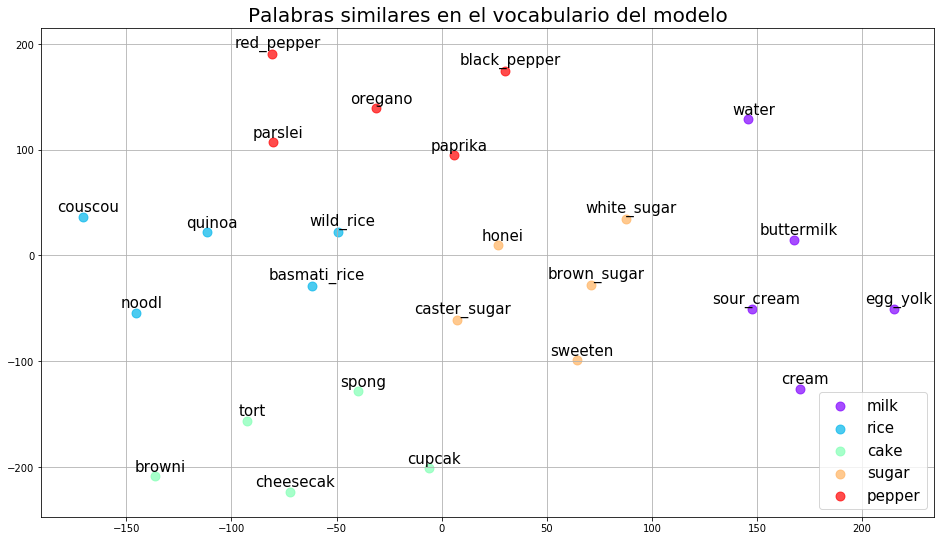
\includegraphics[width=1.0\textwidth]{imagenes/resultados/word-embedding-2.png}
    \caption{Visualización del modelo: elementos similares (ejemplo 1)}
    \label{fig:wordembedding_vis1}
\end{figure} 

En nuestro caso, para analizar la calidad de las representaciones que obtenemos con el modelo de procesamiento de lenguaje vamos a visualizar posibles relaciones de similitud entre palabras del vocabulario del modelo con una de las principales aplicaciones de los modelos de Word Embedding: detectar elementos similares dentro del vocabulario. Esta funcionalidad viene implementada dentro de la librería de Procesamiento de Lenguaje Natural que utilizamos para el entrenamiento y utilización del modelo (\textit{Topic Modelling  Gensim}\footnote{\url{https://radimrehurek.com/gensim/}}). De esta forma, para una palabra dada, podremos obtener aquellas más similares que se encuentren representadas dentro del vocabulario del modelo de lenguaje.

En la Figura \ref{fig:wordembedding_vis1} se pueden ver, para los alimentos \textit{leche}, \textit{arroz}, \textit{tarta}, \textit{azúcar} y \textit{pimiento}, las palabras del vocabulario del modelo más similares para dichos elementos. Como se puede observar, dichas palabras se muestran en inglés tras el proceso de lematización aplicado al conjunto de entrenamiento para la creación del modelo (tal y como se explica en el Capítulo \ref{ch:Capitulo 5}). En dicha figura se muestra cómo, por ejemplo, los elementos más similares a \textit{azúcar} son azúcar moreno, azúcar blanco, endulzar, etc; o cómo para \textit{arroz}, el modelo devuelve \textit{arroz salvaje}, \textit{arroz basmati}, \textit{quinoa} o \textit{couscous}. En este último ejemplo se aprecia la gran potencia que aportan estos modelos, donde detecta que el \textit{couscous} es similar al arroz, llegando a ese punto únicamente a través del modelo predictivo entrenado con las recetas. Con este caso se demuestra cómo el modelo entrenado ha sido capaz de capturar la semántica de los datos con los que se ha entrenado, bajo la idea de que alimentos utilizados en contextos y forma similares, guardan también una relación de parecido. Además, debido a su gran valor en cuanto a similitud, incluso podría ser un sustitutivo del mismo, ya que el uso, preparación, cocinado y combinación con otros ingredientes en recetas es similar entre uno y otro. 

\begin{figure}[H]
    \centering
    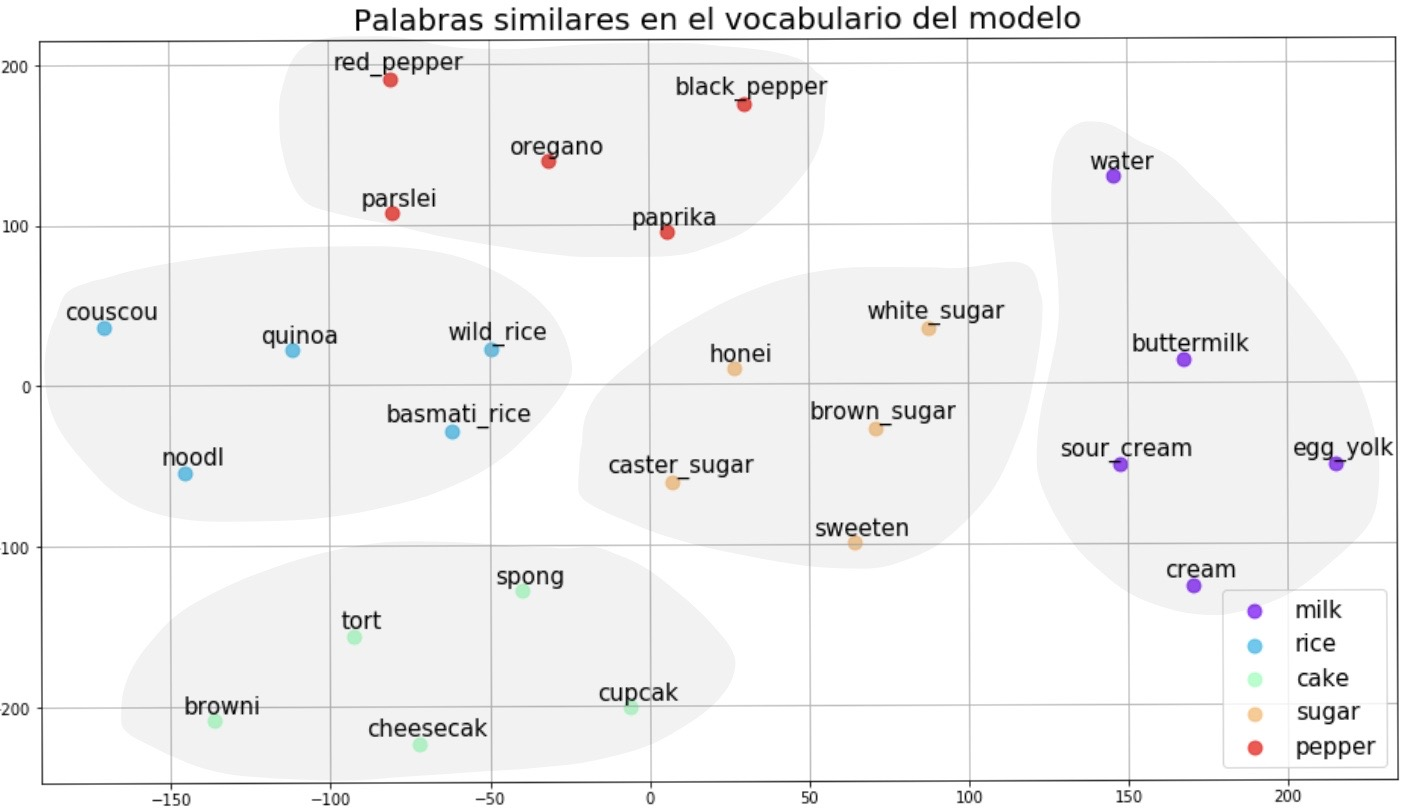
\includegraphics[width=1.0\textwidth]{imagenes/resultados/word-embedding-3.jpg}
    \caption{Visualización del modelo: localización espacial de los items (ej.1)}
    \label{fig:wordembedding_vis2}
\end{figure}


Por otra parte, si en la Figura \ref{fig:wordembedding_vis1} nos fijamos en el vocabulario más similar obtenido para \textit{Leche}, se puede ver cómo se han obtenido como similares \textit{yema de huevo} y \textit{mantequilla}. Esto se puede deber a que gran parte de las recetas que incluyan el ingrediente \textit{leche} sean postres, y aparezca acompañado o con un uso similar a los últimos mencionados. Por ello, es importante hacer ver que las representaciones obtenidas pueden estar sesgadas por las características de las recetas que se utilicen. Aquí se hace necesario utilizar grandes conjuntos de recetas, que permitan abarcar una gran cantidad de combinaciones de ingredientes, así como preparaciones de los mismos, para que el resultado sea lo más realista posible. En este caso, sí podemos concluir que se ha obtenido una buena representación, ya que otro de los elementos más similares es \textit{agua}, lo cual nos permite ver que se están teniendo en cuenta otras características en su representación interna (como en este caso, que es similar a otros elementos del vocabulario que también son bebidas). Además, en dicha imagen se puede ver cómo los elementos similares a cada una de las descripciones textuales elegidas (nombres de alimentos) se encuentran cercanas en cuanto a su representación espacial. Este hecho se aprecia de forma más clara en la Figura \ref{fig:wordembedding_vis2}, donde se han delimitado sobre la imagen aquellos elementos más similares a cada uno de los escogidos.


\begin{figure}[H]
    \centering
    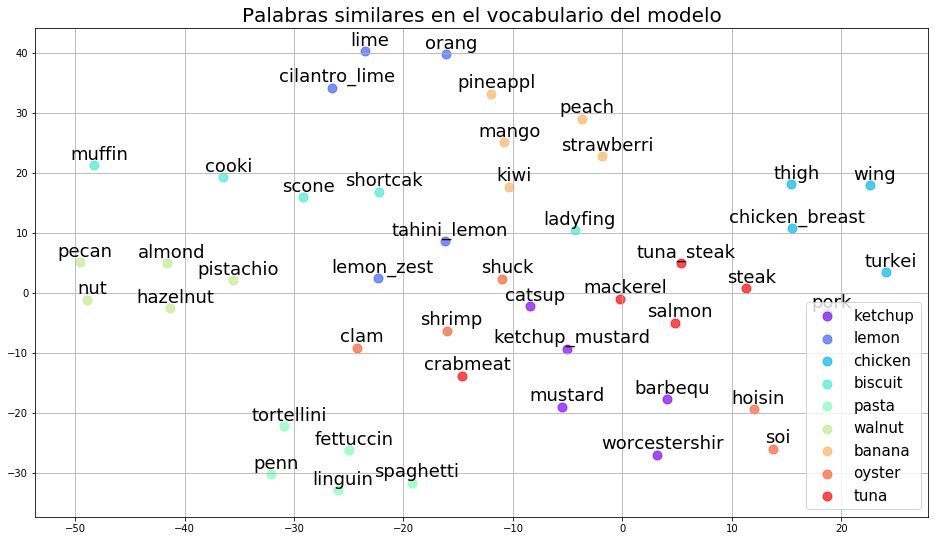
\includegraphics[width=1.0\textwidth]{imagenes/resultados/word-embedding-4.png}
    \caption{Visualización del modelo  (ejemplo 2)}
    \label{fig:wordembedding_vis3}
\end{figure}


Si obtenemos una visualización con mayor número de alimentos, vemos que al aumentar la cantidad de elementos en la visualización no es tan sencillo encontrar una ``separación espacial'' tan clara como la de la Figura \ref{fig:wordembedding_vis2}. Esto se debe a que estamos en un contexto en el que un ingrediente puede tener múltiples usos y en gran cantidad de contextos distintos (p.ej, el limón se utiliza en postres pero también en pescados o carnes). Este hecho se aprecia en la Figura \ref{fig:wordembedding_vis3}. En esta figura podemos contrastar cómo de nuevo, alimentos con usos muy similares son detectados por el modelo sin necesidad de ser el mismo alimento o derivado del mismo: pollo y pavo (a la derecha en azul en la figura) o atún y salmón (en rojo a la derecha), son ejemplos de ello.

Otro caso relevante en el que la semántica de los alimentos ha sido tenida en cuenta dentro del modelo se aprecia en en los elementos similares obtenidos para \textit{Limón} y para \textit{Plátano}. Podemos ver que a pesar de que ambos, \textit{Limón} y \textit{Plátano}, son tipos de frutas, el modelo no se ha limitado a proporcionar como similares otras frutas, sino que en el caso del limón, ha sido capaz de representar características relacionadas con sabores: en este caso, todos los elementos más similares a \textit{Limón} también son cítricos, mientras que en los más parecidos a \textit{Plátano}, no hay ninguno con componente cítrico.

Con estos ejemplos, hemos podido comprobar la calidad de las representaciones obtenidas, puesto que capturan de forma precisa las semejanzas semánticas y sintácticas entre los alimentos, llegando incluso a ser capaz de representar sabores debido a las relaciones intrínsecas entre los alimentos. Estas relaciones se obtienen gracias al conjunto de entrenamiento utilizado que, al ser de instrucciones de preparación de recetas, permiten capturar información del contexto en el que se utilizan dichos alimentos, con cuáles se combinan y qué tipo de preparación y técnicas de cocinado se utilizan en ellos. Además, capturar la semántica de los alimentos en la representación del modelo de lenguaje teniendo en cuenta el uso de los mismos en el ámbito culinario no sólo permite detectar equivalentes, sino que abre una vía hacia la generación, alteración y adecuación de recetas teniendo en cuenta múltiples casuísticas.



\subsection{Resultados del Módulo de Mapeo}\label{sec:res_mapeo}

Tal y como se detalla en el Capítulo \ref{ch:Capitulo 6}, para analizar el funcionamiento de las distintas métricas de distancia utilizadas, se ha realizado un mapeo entre dos bases de datos nutricionales: i-Diet y USDA. Para cada elemento de i-Diet, se aplica el procedimiento de mapeo ya detallado para obtener su equivalente en USDA, utilizando las distintas medidas implementadas. En la Tabla \ref{table8} se pueden ver los resultados alcanzados con estas medidas de distancia. Para una mayor comprensión del modelo, hemos tenido en cuenta distintos niveles de cobertura de los resultados obtenidos. En la columna \textit{Top 1}, se muestra el porcentaje de elementos en la base de datos de i-Diet para los que se ha obtenido el mejor mapeo posible en la base de datos USDA. En el caso de la columna \textit{Top 2}, el valor obtenido se corresponde con el porcentaje de elementos en i-Diet cuyo mejor mapeo posible se encuentra entre los dos mejores resultados obtenidos con el procedimiento, y sucesivamente con el resto de columnas. En dicha tabla, se puede ver cómo las aproximaciones difusas nos permiten obtener los mejores resultados, superando las medidas de distancia semántica, sintáctica, o combinación de ambas. En concreto, la medida de \textit{Distancia difusa entre documentos} nos permite detectar mayor número de equivalencias. En los siguientes apartados se profundiza en los mapeos obtenidos con las distintas métricas para obtener una idea más concreta del comportamiento y eficacia de las mismas.



\setlength{\tabcolsep}{4pt} 
\begin{table}[H]
\small
\begin{tabular}{l|l|l|l|l|l}

\textbf{Medida de distancia} & \textbf{Top 1} &\textbf{Top 2}& \textbf{Top 3} & \textbf{Top 5} & \textbf{Top 10}\\ \hline
Distancia Jaccard & 16.75 & 20.16 & 22.20 & 25.20 & 27.52 \\
Word Mover's Distance & 30.65 & 35.55 & 36.92 & 40.87 & 44.82 \\ \hline
Distancia híbrida & 32.15 & 37.12 & 40.19 & 43.05 & 47.41 \\ \hline 
Distancia Jaccard difusa & 23.84 & 29.70 & 33.37 & 39.23 & 45.64 \\ 
Distancia entre documentos difusa & 35.55 & 40.46 & 43.46 & 47.00 & 53.26 \\ 
\end{tabular}
\caption{Resultados del mapeo ($\%$) con las medidas de distancia}\label{table8}
\end{table}



\subsubsection{Distancia sintáctica entre descripciones}

\begin{flushleft}
    \textit{Distancia de Jaccard}
\end{flushleft}
En la Tabla \ref{table:jaccard} se pueden ver algunos de los mapeos más representativos obtenidos con el procedimiento de mapeo usando la medida de distancia Jaccard. Como ya se ha introducido, esta medida de concordancia utiliza el conjunto de tokens preprocesados obtenidos a partir de cada una de las descripciones alimenticias para asignar un valor de distancia en función de los tokens que pertenecen al conjunto intersección.

\setlength{\tabcolsep}{2pt} 
\begin{table}[H]
\begin{tabular}{p{0.035\textwidth}p{0.24\textwidth}|p{0.26\textwidth}|p{0.27\textwidth}|p{0.10\textwidth}p{0.01\textwidth}}
& \textbf{Alimento a \newline mapear (i-Diet)} & \textbf{Alimento mapeado (USDA)} & \textbf{Mejor mapeo\newline posible (USDA)} & \textbf{Valor\newline distancia} &  \\ \hline

(1) & Peanut oil & Peanut oil & Peanut oil & 0.0 & \textcolor{myGreen}{\cmark} \\ 

(2) & Cauliflower & Cauliflower, raw & Cauliflower, raw & 0.199 & \textcolor{myGreen}{\cmark} \\

(3) & Anchovy &  Anchovy, canned &  Anchovy, canned & 0.125 & \textcolor{myGreen}{\cmark} \\

(4) & Chicory & Brioche & Chicory, beverage & 0.16 & \textcolor{myRed}{\xmark} \\

(5) & Avocado & Vodka & Avocado, raw & 0.33 & \textcolor{myRed}{\xmark} \\

(6) & Swett potatoes & Stewed potatoes & Sweet potato NFS & 0.0 & \textcolor{myRed}{\xmark} \\

\end{tabular}
\caption{\label{table:jaccard} Resultados obtenidos con la distancia de Jaccard}
\end{table}


Esta concordancia a nivel de cadena de caracteres se refleja en los resultados obtenidos, ya que en las tres primeras filas se obtienen mapeos adecuados debido al parecido sintáctico entre los elementos de ambas bases de datos (las descripciones son muy similares desde el punto de vista de caracteres utilizados). De igual forma, se puede apreciar de las filas (3) a (6), puesto que los resultados del mapeo no tienen ningún tipo de relación, más allá de la sintáctica, con los elementos mapeados (además de hacerlo con un valor de distancia mínimo, para nada representativo). A su vez, se puede ver en la fila (6) la falta de robustez con la que contamos con esta métrica, puesto que un mínimo error tipográfico en las descripciones lleva a un mapeo erróneo. 






% \setlength{\tabcolsep}{3pt} 
% \begin{table}[H]
% \begin{tabular}{p{0.045\textwidth}p{0.24\textwidth}|p{0.26\textwidth}|p{0.27\textwidth}|p{0.10\textwidth}p{0.01\textwidth}}
% & \textbf{Alimento a \newline mapear (i-Diet)} & \textbf{Alimento mapeado (USDA)} & \textbf{Mejor mapeo\newline posible (USDA)} & \textbf{Valor\newline distancia} &  \\ \hline

% (1) &  &  &  & & \cmark \\ 

% (2) &  &  &  & & \cmark \\

% (3) &  &  &  & & \cmark \\

% (4) &  &  &  & & \xmark \\

% (5) &  &  &  & & \xmark \\

% (6) &  &  &  & & \xmark \\

% \end{tabular}
% \end{table}

\subsubsection{Distancia semántica entre descripciones}
\begin{flushleft}
    \textit{Distancia Word Mover's }
\end{flushleft}% \subsubsection{Word Mover's Distance}

Dado que no siempre vamos a contar con descripciones muy similares para elementos equivalentes, utilizar la semántica intrínseca en estas descripciones puede ayudar a obtener mejores resultados (tal y como se puede observar en la Tabla \ref{table8}). En el caso de la distancia \textit{Word Mover's}, en la Tabla \ref{table:wmd} se pueden ver algunos de los mapeos más representativos obtenidos con esta métrica. 

\setlength{\tabcolsep}{2pt} 
\begin{table}[H]
\begin{tabular}{p{0.035\textwidth}p{0.24\textwidth}|p{0.26\textwidth}|p{0.27\textwidth}|p{0.10\textwidth}p{0.01\textwidth}}
& \textbf{Alimento a \newline mapear (i-Diet)} & \textbf{Alimento mapeado (USDA)} & \textbf{Mejor mapeo\newline posible (USDA)} & \textbf{Valor\newline distancia} &  \\ \hline

(1) & Sweet wine & Wine, dessert, sweet & Wine, dessert, sweet & 13.207 & \textcolor{myGreen}{\cmark} \\ 

(2) & Tomato paste & Tomato, catsup & Tomato, catsup & 15.453 & \textcolor{myGreen}{\cmark} \\

(3) & Pate liver not specified & Liver paste or pate, chicken & Liver paste or pate, chicken & 17.555 & \textcolor{myGreen}{\cmark} \\

(4) & Sausage Bratwurst & Deer Sausage & Bratwurst & 10.043 & \textcolor{myRed}{\xmark} \\

(5) & Cocoa and hazelnut butter, Nocilla, Nutela & Almond Butter & No matches & 19.028 & \textcolor{myRed}{\xmark} \\

(6) & Sobrasada mallorquina & No matches & No matches & $\infty$ & \textcolor{myRed}{\xmark} \\
\end{tabular}
\caption{\label{table:wmd} Resultados obtenidos con la distancia de Word's Mover}
\end{table}

Además de poder resolver sin problema mapeos donde las descripciones son similares (véase fila (1) en la Tabla \ref{table:wmd}), también es capaz de solventar otros casos con una mayor dificultad, como puede ser el mapeo mostrado en la fila (2) de dicha tabla. En este caso podemos ver, cómo a pesar de utilizar una marca alimenticia, el mapeo se resuelve de forma correcta. Este ejemplo tiene una alta relevancia, ya que estamos mapeando bases de datos de distintas culturas culinarias y las marcas comerciales no tienen por qué coincidir en ambas zonas geográficas. Con las representaciones del modelo de Word Embedding estamos consiguiendo lidiar con esta complejidad añadida.

Otro detalle destacable es el que se expone en los ejemplos (4) y (5), donde se puede apreciar que en ambas bases de datos, existen distintos niveles de detalle en las descripciones de los alimentos, lo que añade más complejidad al problema de mapeo. Si nos fijamos en estos ejemplos, uno resulta en un mapeo correcto mientras que el otro no, y a pesar de ello, los valores de distancia obtenidos no resultan esclarecedores como para poder determinar una relación entre valor de distancia y precisión el mapeo. Aquí aparece la necesidad de lidiar con la vaguedad del lenguaje que estas diferencias de detalle provocan, para así poder aumentar la robustez y precisión de la tarea de mapeo. Tal y como se detallará más adelante en este capítulo, para lidiar con este tipo de obstáculos se hará uso de una aproximación difusa de esta medida de distancia. 




Por otra parte, con el ejemplo en la fila (5) se remarca de nuevo cómo el uso de modelos de Word Embedding pueden permitir detectar posibles equivalencias, como es este caso, el cual es especialmente interesante, puesto que en USDA no hay ningún mapeo posible (debido a las diferencias culturales en la cocina). Por último, destacar el ejemplo en la fila (6), donde el elemento a mapear no está traducido al idioma en el que hemos implementado el modelo de Procesamiento de Lenguaje Natural. En este caso, esto supone un problema añadido a la hora de realizar el mapeo, porque el uso de malas traducciones empobrecen las representaciones que podamos obtener.



\subsubsection{Distancia híbrida entre descripciones}

En vista a mejorar los resultados obtenidos con las métricas previas, se ha diseñado una medida que tiene en cuenta ambas aproximaciones a través de una combinación ponderada de las medidas Jaccard y Word's Mover. 

\setlength{\tabcolsep}{4pt} 
\begin{table}[H]
\centering
\begin{tabular}{p{0.05\textwidth}c|c|c|c|c|c} 
& \textbf{w} & \textbf{Top 1}& \textbf{Top 2} & \textbf{Top 3} & \textbf{Top 5} & \textbf{Top 10} \\ \hline
(1)& 1.0 & 16.75 & 20.16 & 22.20 & 25.20 & 27.52 \\
(2)& 0.0 &  30.65 & 35.55 & 36.92 & 40.87 & 44.82 \\
(3)& 0.6 &  25.06 & 29.01 & 30.92 & 33.51 & 37.87 \\
(4)& 0.55 &  25.88 & 29.70 & 31.88 & 35.42 & 39.23 \\
(5)& 0.5 &  26.83 & 30.79 & 33.10 & 36.23 & 41.82 \\
(6)& 0.45 &  27.79 & 31.60 & 33.65 & 39.64 & 44.14 \\
(7)& 0.4 &  29.42 & 34.46 & 36.23 & 41.82 & 46.18 \\
(8)& 0.35 &  30.38 & 35.55 & 37.46 & 42.23 & 46.73 \\
(9)& 0.3 &  31.60 & 36.23 & 38.82 & 43.18 & 47.00 \\
\textcolor{UniBlue}{\textbf{(10)}}& \textcolor{UniBlue}{\textbf{0.25}}  & \textcolor{UniBlue}{\textbf{32.01}} & \textcolor{UniBlue}{\textbf{37.32}} & \textcolor{UniBlue}{\textbf{38.82}} & \textcolor{UniBlue}{\textbf{42.64}}  & \textcolor{UniBlue}{\textbf{47.13}} \\
(11)& 0.20 & 32.15 & 37.19 & 40.19 & 43.05 & 46.59 \\
(12)& 0.15 & 32.69 & 37.05 & 40.05 & 42.37 & 46.59 

\end{tabular}
\caption{\label{table:hybrid} Resultados obtenidos con la distancia híbrida}
\end{table}

En la Tabla \ref{table:hybrid} se puede ver la experimentación realizada con esta medida híbrida, teniendo en cuenta ambas métricas en diferentes proporciones. La prueba (10), destacada en azul, es la que en vista a los resultados, ofrece los mapeos de mejor calidad de entre todas las combinaciones. 

En la Figura \ref{fig:plot_w} se aprecia la información de la Tabla \ref{table:hybrid}. En esta figura se muestra la eficacia de los mapeos alcanzados con la distancia híbrida en función del valor asociado al parámetro \textit{w}. Tal y como se observa, la calidad de los mapeos solo mejora cuando se tiene en cuenta de forma mínima la información sintáctica obtenida con la distancia de Jaccard (ponderada por el valor del parámetro \textit{w}), resultando contraproducente en la mayor parte de los resultados obtenidos. Sin embargo, los resultados obtenidos con esta medida híbrida dejan ver que ponderar la información sintáctica y semántica no obtiene resultados destacables, puesto que el aumento de los porcentajes de acierto no es muy representativo, sobre todo si los comparamos con los obtenidos con la métrica \textit{Word Mover's Distance}. 

\begin{figure}[H]
    \centering
    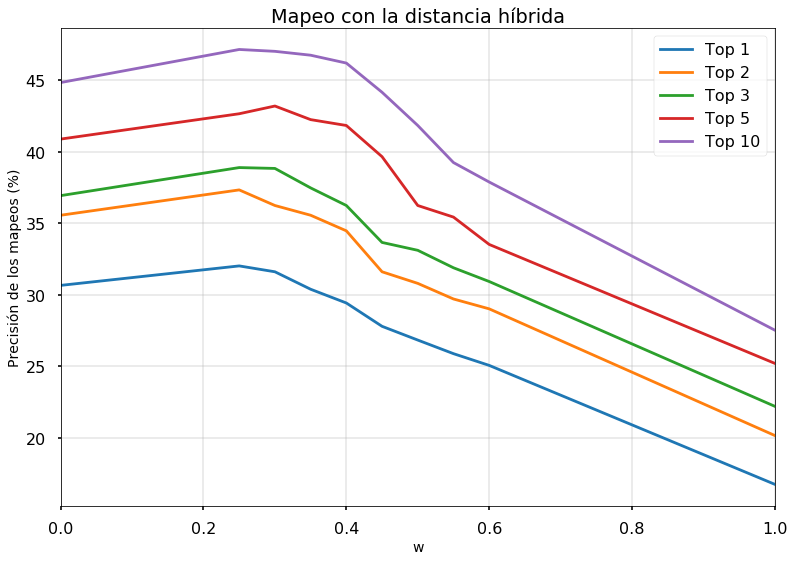
\includegraphics[width=0.8\textwidth]{imagenes/resultados/plot/rr.png}
    \caption{Medida de distancia híbrida: comportamiento del parámetro w }
    \label{fig:plot_w}
\end{figure}


\subsubsection{Medidas de distancia difusas}

Tal y como se ha podido ver en los resultados alcanzados con las métricas anteriores, se hace necesario involucrar otras técnicas que permitan un tratamiento de la información textual capaz de lidiar con distintos niveles de detalle en las descripciones, así como con la ambigüedad intrínseca del lenguaje para poder llevar a cabo un procedimiento de mapeo más robusto. En este caso, tal y como se comentó previamente, se han obtenido versiones difusas de Jaccard y de Word Mover's. 

\begin{flushleft}
   \textit{Jaccard difuso}
\end{flushleft}
% \subsubsection{Jaccard difuso}

Como se ha podido observar en la Tabla \ref{table8}, los resultados obtenidos con la medida de Jaccard difusa mejoran los conseguidos con la versión clásica, debido a una mayor permisividad al considerar que los elementos que se comparen no tienen por qué ser exactamente iguales a la hora de detectar equivalencias (aunque sí suficientemente parecidos). Sin embargo, a pesar de obtener mejores resultados que con la distancia de Jaccard, sigue habiendo una fuerte dependencia entre el parecido de palabras concretas entre las descripciones, como se puede apreciar en la fila (4) en la Tabla \ref{table:jac_fuzzy}, que muestra algunos de los mapeos obtenidos con la medida difusa de Jaccard. Esto es debido en su mayoría a las implicaciones que conlleva trabajar con descripciones sintácticas a la hora de detectar posibles equivalencias.

\setlength{\tabcolsep}{2pt} 
\begin{table}[H]
\begin{tabular}{p{0.035\textwidth}p{0.24\textwidth}|p{0.26\textwidth}|p{0.27\textwidth}|p{0.10\textwidth}p{0.01\textwidth}}
& \textbf{Alimento a \newline mapear (i-Diet)} & \textbf{Alimento mapeado (USDA)} & \textbf{Mejor mapeo\newline posible (USDA)} & \textbf{Valor\newline distancia} &  \\ \hline

(1) & Avocado & Avocado, raw & Avocado, raw & 0.5 & \textcolor{myGreen}{\cmark} \\ 

(2) & Watercress & Watercress, raw & Watercress, raw & 0 & \textcolor{myGreen}{\cmark} \\

(3) & Crab & Crab, cooked, NS as to cooking method & Crab, cooked, NS as to cooking method & 0.333 & \textcolor{myGreen}{\cmark} \\

(4) & Soybean sprouts & Sprouts, NFS & Bean sprouts, raw & 0.666 & \textcolor{myRed}{\xmark} \\

(5) & Broccoli & Licorice & Broccoli, raw & 0.16 & \textcolor{myRed}{\xmark} \\

(6) & Peanut, roasted & Peanuts, honey roasted & Peanuts, roasted, salted & 0.333 & \textcolor{myRed}{\xmark} \\

\end{tabular}
\caption{\label{table:jac_fuzzy} Resultados obtenidos con la distancia de Jaccard difusa}
\end{table}



\begin{flushleft}
    \textit{Distancia difusa entre documentos}
\end{flushleft}
% \subsubsection{Distancia difusa entre documentos}

En vista a los resultados obtenidos con esta medida de distancia (ver Tabla \ref{table8}), con esta medida es con la que alcanzamos los mejores resultados. Esto se debe mayoritariamente a que con las medidas detalladas hasta ahora, se le da mucha importancia a cada elemento considerado dentro de la descripción, ya que todas las palabras tienen la misma importancia en la descripción global. Sin embargo, si nos referimos al procesamiento de lenguaje natural, suponer que cada elemento de la descripción tiene la misma relevancia no es una buena práctica, ya que favorece a evaluar la similitud entre descripciones valorándola elemento a elemento y no como un todo. Con esta métrica le estamos dando mayor importancia al conjunto en sí, puesto que a la hora de calcular el papel que tiene cada elemento en la descripción, lo hacemos en función de su parecido semántico con la otra descripción a un nivel global. Con ello, permitimos una mayor flexibilidad a la hora de encontrar equivalencias en la base de datos. 


Resultados concretos con esta medida de distancia se pueden ver en la Tabla \ref{table:ddd}. En términos generales, se puede observar cómo se obtiene mayor rigor con esta técnica, pues mejora mapeos erróneos vistos en apartados anteriores (como en las filas 1 y 5). Además, se ha observado un comportamiento generalizado en las correspondencias obtenidas, y es que mantiene la semántica de los elementos a mapear. Con ello nos referimos a que con la semántica capturada con el modelo somos capaces de identificar los alimentos a nivel de ingrediente o alimento principal en la descripción y las dificultades que obtenemos se deben en su mayoría a los problemas derivados de distintos niveles de detalle entre ambas bases de datos. Esto es lo ocurre con el mapeo (4) y (5) en la Tabla \ref{table:ddd}. Esto último es relevante en nuestro problema a resolver, puesto que esta semántica intrínseca nos permitirá detectar alimentos equivalentes entre sí cuando queramos modificar alimentos concretos de las recetas.


    
\setlength{\tabcolsep}{2pt} 
\begin{table}[H]
\begin{tabular}{p{0.035\textwidth}p{0.24\textwidth}|p{0.26\textwidth}|p{0.27\textwidth}|p{0.10\textwidth}p{0.01\textwidth}}
& \textbf{Alimento a \newline mapear (i-Diet)} & \textbf{Alimento mapeado (USDA)} & \textbf{Mejor mapeo\newline posible (USDA)} & \textbf{Valor\newline distancia} &  \\ \hline

(1) & Sausage Bratwurst & Bratwurst & Bratwurst & 0.5 & \textcolor{myGreen}{\cmark} \\ 

(2) & Chicory & Chicory beverage & Chicory beverage & 0.285 & \textcolor{myGreen}{\cmark} \\

(3) & Chocolate and cream pudding, Chamburcy & Pie, chocolate cream & Pie, chocolate cream & 0.555 & \textcolor{myGreen}{\cmark} \\

(4) & Swett potatoes & Potato, NFS & Sweet potato NFS & 0.0 & \textcolor{myRed}{\xmark} \\

(5) & Cocoa and hazelnut butter, Nocilla, Nutela & Hazelnuts & No matches & 0.8 & \textcolor{myRed}{\xmark} \\

(6) & Sobrasada mallorquina & No matches & No matches & $\infty$ & \textcolor{myRed}{\xmark} \\

\end{tabular}

\caption{\label{table:ddd} Resultados obtenidos con la distancia entre documentos difusos}
\end{table}

Por último, respecto a los valores de precisión obtenidos con esta métrica (ver \ref{table8}), debemos tener en cuenta que los resultados son de suficientemente calidad y coherencia teniendo en cuenta que el modelo de procesamiento de lenguaje natural utilizado se basa en aprendizaje predictivo no supervisado. Para comprender la calidad de los resultados obtenidos, hay que valorar que el procedimiento de mapeo obtiene para cada uno de los elementos de i-Diet, el mejor mapeo posible de entre todos los elementos en USDA (un total de 8606), realizando el cálculo de distancia para todos los posibles emparejamientos. Si nos fijamos en las columnas \textit{Top 10}, estas demuestran la tendencia a que a mayor flexibilidad en la medida de precisión utilizada seguimos siendo capaces de encontrar mapeos adecuados, y que el acierto en el mapeo no es fruto del azar. 

\subsubsection{Comparativa entre medidas difusas y no difusas}

Tal y como se observó anteriormente, los mapeos obtenidos con las medidas de distancia Jaccard y Word's Mover son mejorados por sus respectivas versiones difusas (ver Tabla \ref{table8}).

Si nos centramos exclusivamente en el caso de Jaccard, esta mejora se debe principalmente a que los mapeos obtenidos con la medida clásica de Jaccard se basan en la comparación íntegra de las descripciones desde un punto de vista morfológico. Con su versión difusa se valoran las descripciones con un mayor grado de flexibilidad, permitiendo así que el alimento principal que aparece en las descripciones se mantenga en los mapeos resultantes. Este hecho se puede apreciar en la Tabla \ref{tab:crisp-fuzzy-jaccard}, la cual recoge una comparativa de algunos mapeos obtenidos con ambas versiones (Jaccard y Jaccard difuso). En dicha tabla podemos ver cómo en las correspondencias obtenidas con la versión difusa se mantiene el concepto de \textit{Aceite}. Sin embargo, con la versión clásica de Jaccard, se tiende a proporcionar un mapeo con el ingrediente mayoritario, lo cual no tiene que derivar en un mapeo correcto (que en este caso, sería el vegetal del que se obtiene dicho aceite).

\begin{table}[H]

\begin{tabular}[c]{p{0.02\textwidth}|p{0.17
\textwidth}|p{0.17\textwidth}|p{0.20\textwidth}|p{0.17\textwidth}|p{0.18\textwidth}p{0.01\textwidth}}
 & \textbf{Alimento a} \newline \textbf{mapear (i-Diet)} & \begin{tabular}[c]{@{}l@{}}\\\textbf{Top 1} \end{tabular} &  \begin{tabular}[c]{@{}l@{}}\\\textbf{Top 2} \end{tabular} &  \begin{tabular}[c]{@{}l@{}}\\\textbf{Top 3} \end{tabular} & \textbf{Mejor mapeo posible (USDA)} & \\ \hline

$J$ & Peanut oil & Peanut oil & Peanut, boiled & Tuna pot pie & Peanut oil & \textcolor{myGreen}{\cmark} \\

$\tilde{J}$ & Peanut oil & Peanut oil & Walnut oil & Flaxseed oil & Peanut oil & \textcolor{myGreen}{\cmark} \\ \hline

$J$ & Wheat germ oil & Wheat germ oil & Wheat germ, plain & Roll, whole grain white & Wheat germ oil & \textcolor{myGreen}{\cmark} \\

$\tilde{J}$ & Wheat germ oil &  Wheat germ oil & Sunflower oil & Sesame oil & Wheat germ oil  & \textcolor{myGreen}{\cmark} \\ \hline

$J$ & Sunflower oil & Sunflower oil & Sunfloweer seeds, NFS, & Safflower oil & Sunflower oil & \textcolor{myGreen}{\cmark} \\

$\tilde{J}$ & Sunflower oil & Sunflower oil & Soybean and sunflower oil & Canola,\newline soybean and sunflower oil & Sunflower oil & \textcolor{myGreen}{\cmark} \\

\end{tabular}
\caption{\label{tab:crisp-fuzzy-jaccard} Comparación entre Jaccard ($J$) y Jaccard difuso ($\tilde{J}$) }
\end{table}


En el caso de Word Mover's, debemos valorar que la métrica computa la distancia de cada elemento en una descripción hacia el elemento más parecido en la otra descripción. Con la versión difusa que hemos diseñado inspirándonos en esta medida, valoramos el parecido de cada elemento al conjunto de la intersección generado por ambas descripciones. Esto nos permite valorar la distancia de los elementos hacia descripciones completas, para así valorar las ambigüedades y características propias del lenguaje natural presentes en ellas. En la Tabla \ref{tab:crisp-fuzzy-documents} se puede apreciar el efecto de considerar la descripción de forma más global. En los ejemplos de dicha tabla, se puede ver cómo los mapeos alcanzados con la medida de distancia difusa entre documentos ($\tilde{D}$) proporciona resultados de más calidad.








\begin{table}[H]

\begin{tabular}[c]{p{0.1\textwidth}|p{0.14
\textwidth}|p{0.17\textwidth}|p{0.20\textwidth}|p{0.17\textwidth}|p{0.15\textwidth}p{0.01\textwidth}}
 & \textbf{Alimento} \newline \textbf{amapear\newline
 (i-Diet)} & \begin{tabular}[c]{@{}l@{}}\\\textbf{Top 1} \end{tabular} &  \begin{tabular}[c]{@{}l@{}}\\\textbf{Top 2} \end{tabular} &  \begin{tabular}[c]{@{}l@{}}\\\textbf{Top 3} \end{tabular} & \textbf{Mejor mapeo posible (USDA)} & \\ \hline

$WMD$ & Cherry & Chips, rice & Cherries, dried & Ceviche & Cherry & \textcolor{myRed}{\xmark} \\

$\tilde{D}$ & Cherry & Cherries, frozen & Cherries, dried & Cobbler, cherry & Cherry & \textcolor{myGreen}{\cmark} \\ \hline

$WMD$ & Garlic & Garlic, raw & Roll, garlic & Garlic, sauce & Garlic, raw & \textcolor{myGreen}{\cmark} \\

$\tilde{D}$ & Garlic & Garlic, sauce & Garlic, sauce & Garlic, cooked & Garlic, raw & \textcolor{myRed}{\xmark} \\ \hline

$WMD$ & Lemon & Lo mein,\newline NFS & Salmon, smoked & Lo mein, with beef   & Lemon, raw & \textcolor{myRed}{\xmark} \\

$\tilde{D}$ & Lemon   & Lemon, raw & Cassaba melon, raw & Lemon butter sauce & Lemon, raw & \textcolor{myGreen}{\cmark} \\

\end{tabular}
\caption{\label{tab:crisp-fuzzy-documents} Comparación entre Word Mover's (\textit{WMD}) y Distancia difusa entre documentos ($\tilde{D}$) }
\end{table}


\subsubsection{Otras medidas de distancia}

% Se han hecho experimentos adicionales 
% Se han utilizado otras medidas de distancia pero no han funcionado y por eso no se entra en detalle. 
Además de las medidas de distancia ya comentadas en esta sección, también se hecho experimentos adicionales con otras medidas de distancia. Este es el caso de la medida de distancia sintáctica Levenshtein, así como otras pruebas híbridas combinando las medidas difusas. Con estas métricas, no se han obtenido resultados relevantes que añadan detalles adicionales a lo explicado en apartados anteriores, por lo que no se entra en detalle en este capítulo.

\subsubsection{Influencia del Word Embedding utilizado}\label{WordEmbedding}

Los resultados obtenidos con el procedimiento de mapeo también nos pueden ayudar a analizar la eficacia de utilizar un Word Embedding específico para este problema y no uno genérico ya entrenado (tal y como se mostró en el Capítulo \ref{ch:Capitulo 5}). En la Tabla \ref{tablecomp} se muestra el porcentaje de acierto de los mapeos obtenidos con un modelo de Word Embedding específico (el entrenado por nosotros) y uno genérico (un modelo de Word Embedding entrenado con el conjunto de datos de Google News). Para ello, se ha utilizado la medida de distancia con mejor comportamiento (distancia de documentos difusos). 

\setlength{\tabcolsep}{4pt} 
\begin{table}[H]
\centering
\begin{tabular}{l|l|l|l|l|l}
\textbf{Modelo de W.E.} & \textbf{Top 1} &\textbf{Top 2}& \textbf{Top 3} & \textbf{Top 5} & \textbf{Top 10}\\ \hline
W.E. Google & 5.85 & 6.26 & 6.40 & 7.22 & 7.76 \\
W.E. Recetas & 35.55 & 40.46 & 43.46 & 47.00 & 53.26 \\ 
\end{tabular}
\caption{Resultados del mapeo ($\%$) para distintos modelos de W.E.}\label{tablecomp}
\end{table}


En la Figura \ref{fig:comp} se pueden ver los resultados de la Tabla \ref{tablecomp}. Con ella, podemos ratificar que el uso de un modelo específico en este problema es lo que nos ha llevado a obtener buenas representaciones (y por tanto mapeos) que no podríamos haber obtenido con uno genérico.

\begin{figure}[H]
    \centering
    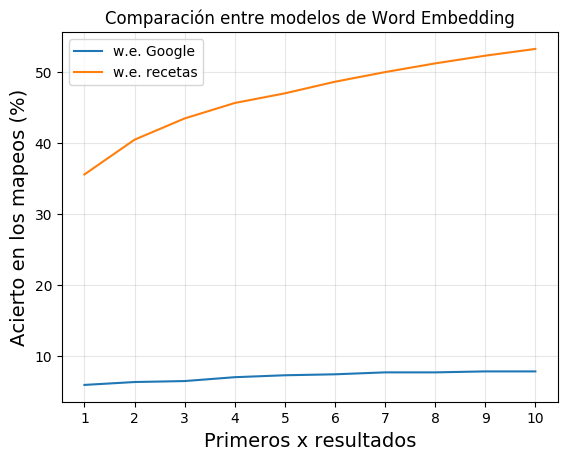
\includegraphics[width=0.80\textwidth]{imagenes/resultados/plot/xx.png}
    \caption{Comparación entre Word Embedding genéricos y preentrenados}
    \label{fig:comp}
\end{figure}




\section{Resultados del Módulo de Consultas Adaptadas}\label{sec:res_adap}

Para poder analizar los resultados obtenidos con este módulo, en este apartado se muestran algunos ejemplos representativos de adaptaciones de recetas visualizadas a través del prototipo de la aplicación. En primer lugar, vamos a ver cómo se comporta el sistema de adaptación de recetas con las restricciones incorporadas en el sistema. Para ello, se va a ilustrar con una receta cuyos ingredientes no satisfacen ni la dieta vegetariana ni la vegana (ver Figura \ref{fig:ejemplo8}). Tal y como se muestra en la Figura \ref{fig:ejemplo7}, el módulo de Consultas Adaptadas es capaz de detectar aquellos ingredientes no aptos para una dieta vegetariana (en este caso, el ingrediente \textit{Bacon)}. De igual forma ocurre con la opción vegana, cuyos ingredientes no veganos son detectados también a través del módulo de Consultas Adaptadas (ver Figura \ref{fig:ejemplo6}).


\begin{figure}[H]
    \centering
    \begin{subfigure}[b]{0.31\linewidth}
        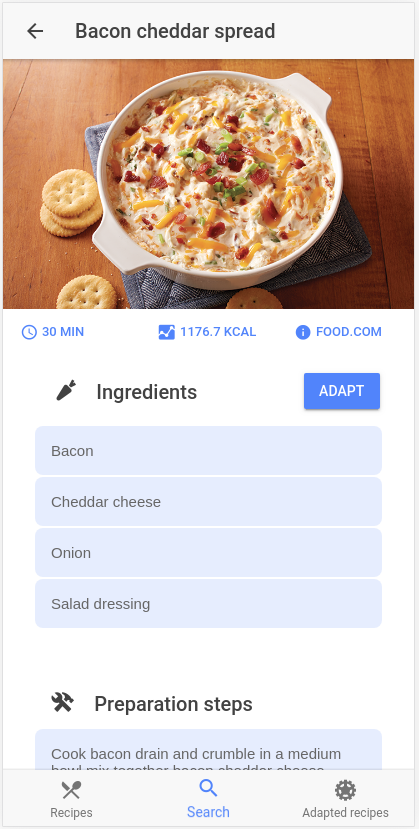
\includegraphics[width=\linewidth]{imagenes/app/pantallas/ejemplo8.png}
        \caption{Receta original}
        \label{fig:ejemplo8}
    \end{subfigure}
    \begin{subfigure}[b]{0.308\linewidth}
        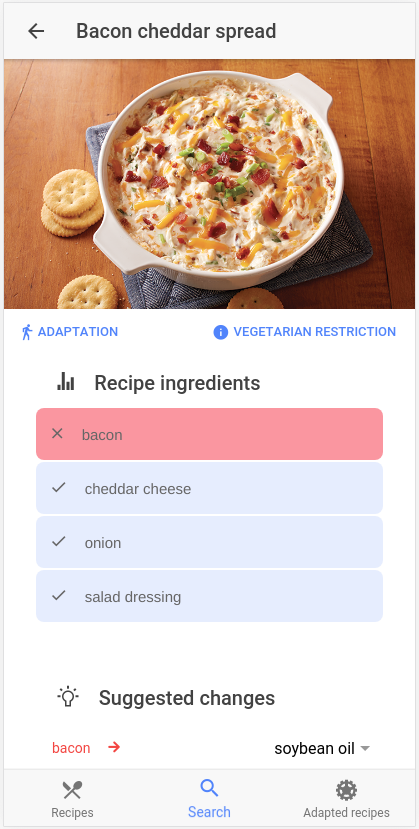
\includegraphics[width=\linewidth]{imagenes/app/pantallas/ejemplo7.png}
        \caption{Opción vegetariana}
        \label{fig:ejemplo7}
    \end{subfigure}
    \begin{subfigure}[b]{0.31\linewidth}
        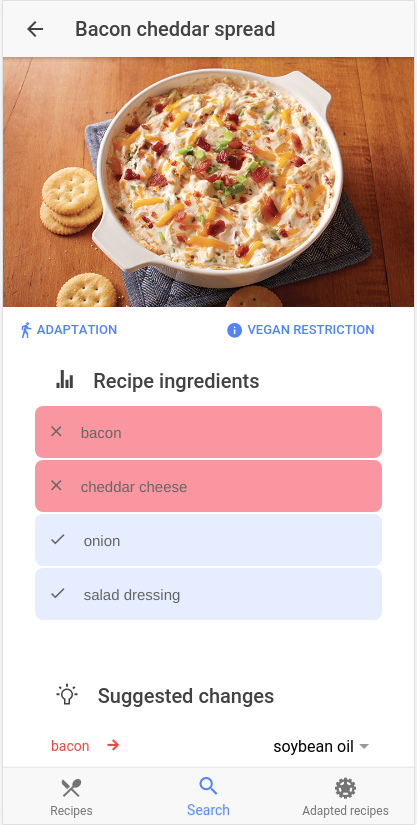
\includegraphics[width=\linewidth]{imagenes/app/pantallas/ejemplo6.png}
        \caption{Opción vegana}
        \label{fig:ejemplo6}
    \end{subfigure}
    \caption{Adaptación de recetas a restricciones vegetarianas y veganas}
    \label{fig:todos}
\end{figure} 

Si nos centramos en adaptaciones a dietas veganas, en la Figura \ref{fig:ejemplo1} se puede ver una receta con ingredientes no compatibles con dicha dieta. De hecho, al aplicar la restricción de dieta vegana (ver Figura \ref{fig:ejemplo2}), podemos ver cómo el sistema evalúa correctamente los ingredientes al detectar aquellos no compatibles con la restricción. Si modificamos el ingrediente no compatible (en este caso es \textit{Mantequilla}), se facilitan algunas alternativas para poder sustituir dicho ingrediente. Podemos observar en la Figura \ref{fig:ejemplo3} algunas de las opciones para reemplazar la mantequilla: entre ellas, se propone la mantequilla vegetal, la cual es apta para estas dietas. Sin embargo, no siempre obtenemos adaptaciones adecuadas para las recetas. Un ejemplo de ello ocurre con la receta mostrada en la Figura \ref{fig:ejemplo10}. Tal y como se detecta con el módulo de Consultas Adaptadas, esta receta contiene \textit{Leche}, ingrediente no apto para una receta vegana (ver Figura \ref{fig:ejemplo11}). Sin embargo, ninguna las alternativas propuestas es adecuada para la receta en cuestión (ver Figura \ref{fig:ejemplo12}). Esto se debe a que no siempre se consigue un alimento alternativo totalmente adecuado para la receta, más aún si se trata de restricciones tan estrictas que limitan los alimentos permitidos a un conjunto muy escaso que impide encontrar opciones que mantengan la esencia del plato.


\begin{figure}[H]
    \centering

    \begin{subfigure}[b]{0.30\linewidth}
        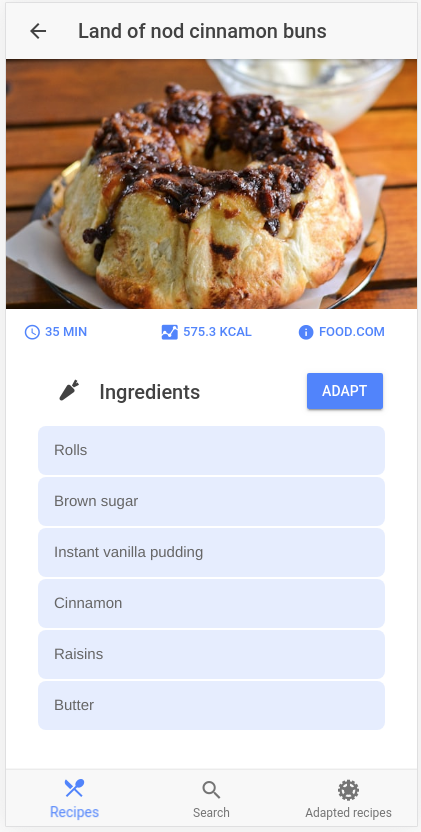
\includegraphics[width=\linewidth]{imagenes/app/pantallas/ejemplo1.png}
        \caption{Receta original}
        \label{fig:ejemplo1}
    \end{subfigure}
    \begin{subfigure}[b]{0.303\linewidth}
        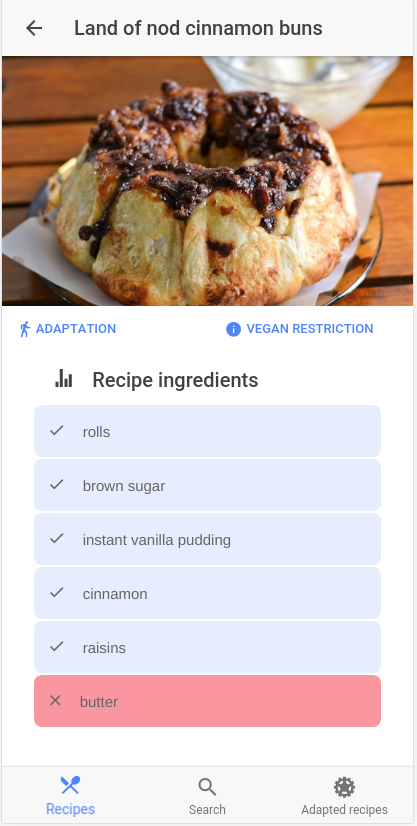
\includegraphics[width=\linewidth]{imagenes/app/pantallas/ejemplo2.png}
        \caption{Adaptando receta I}
        \label{fig:ejemplo2}
    \end{subfigure}
    \begin{subfigure}[b]{0.30\linewidth}
        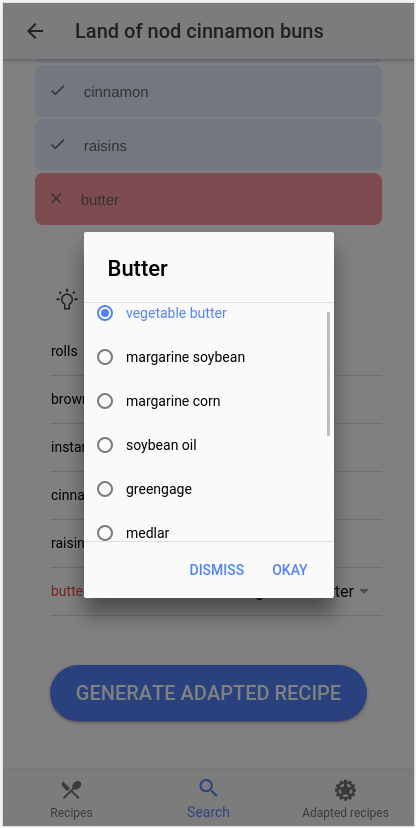
\includegraphics[width=\linewidth]{imagenes/app/pantallas/ejemplo3.png}
        \caption{Adaptando receta II}
        \label{fig:ejemplo3}
    \end{subfigure}
    \caption{Adaptación de una receta vegana I}
    \label{fig:seleccion1}
\end{figure} 

\begin{figure}[H]
    \centering
    \begin{subfigure}[b]{0.30\linewidth}
        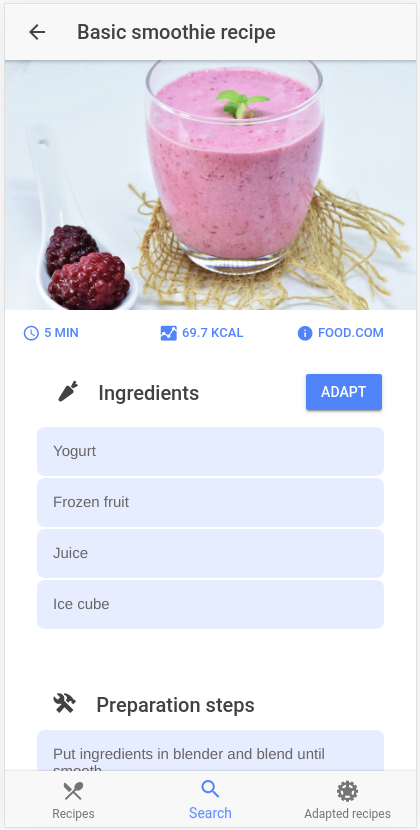
\includegraphics[width=\linewidth]{imagenes/app/pantallas/ejemplo10.png}
        \caption{Receta original}
        \label{fig:ejemplo10}
    \end{subfigure}
    \begin{subfigure}[b]{0.301\linewidth}
        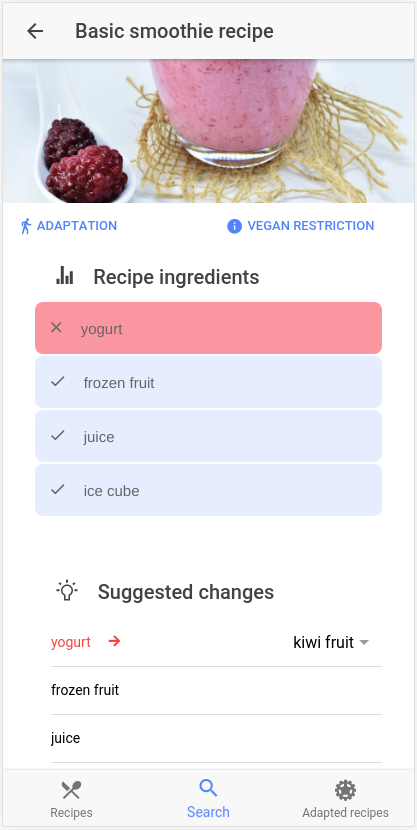
\includegraphics[width=\linewidth]{imagenes/app/pantallas/ejemplo11.png}
        \caption{Adaptando receta I}
        \label{fig:ejemplo11}
    \end{subfigure}
    \begin{subfigure}[b]{0.299\linewidth}
        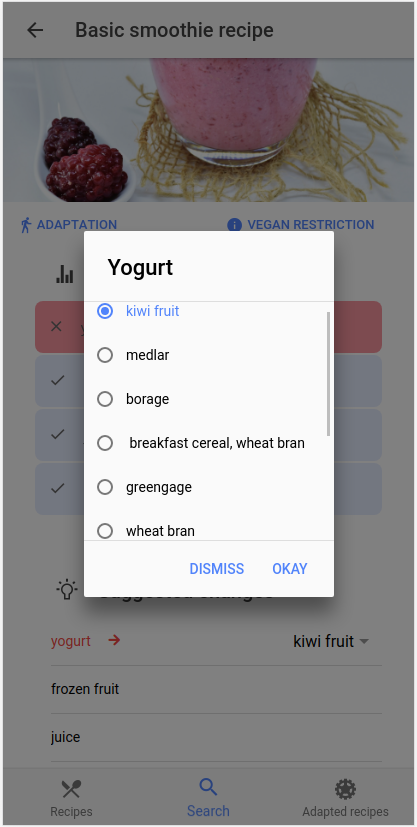
\includegraphics[width=\linewidth]{imagenes/app/pantallas/ejemplo12.png}
        \caption{Adaptando receta II}
        \label{fig:ejemplo12}
    \end{subfigure}
    \caption{Adaptación de una receta vegana II}
    \label{fig:seleccion3}
\end{figure}


Por último, en las Figuras \ref{fig:ejemplo13}, \ref{fig:ejemplo14} y \ref{fig:ejemplo15} se muestra un ejemplo de adaptación sujeta a las restricciones de la
receta vegetariana. Se puede ver que los elementos que se deben adecuar a dicha dieta son       detectados correctamente (en este caso el ingrediente \textit{Pollo)}, y algunas de las sugerencias para su sustitución. Se puede apreciar que las alternativas son coherentes, puesto que se sugiere utilizar verdura o incluso algún tipo de fruta en su lugar, los cuales son substitutos bastante intuitivos para esta dieta.

\begin{figure}[H]
    \centering
    \begin{subfigure}[b]{0.31\linewidth}
        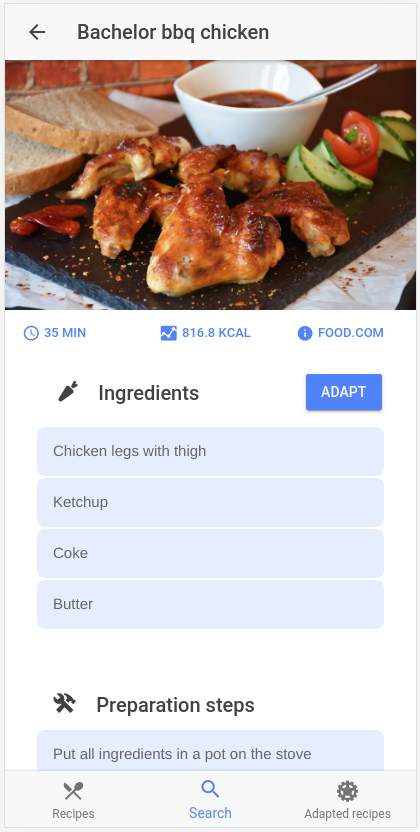
\includegraphics[width=\linewidth]{imagenes/app/pantallas/ejemplo13.png}
        \caption{Receta original}
        \label{fig:ejemplo13}
    \end{subfigure}
    \begin{subfigure}[b]{0.31\linewidth}
        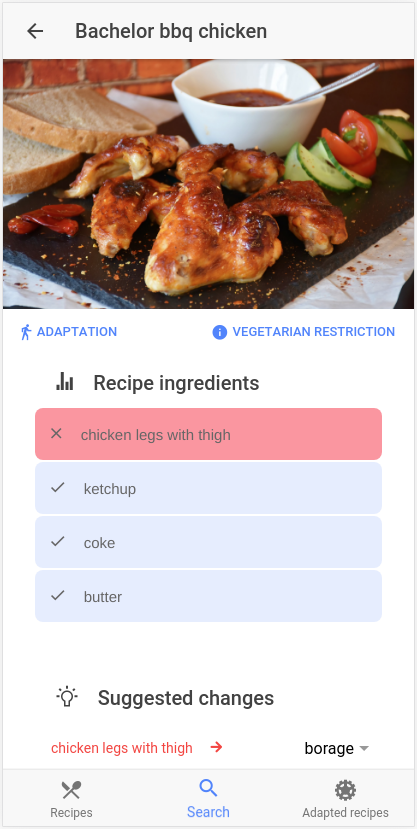
\includegraphics[width=\linewidth]{imagenes/app/pantallas/ejemplo14.png}
        \caption{Adaptando receta I}
        \label{fig:ejemplo14}
    \end{subfigure}
    \begin{subfigure}[b]{0.31\linewidth}
        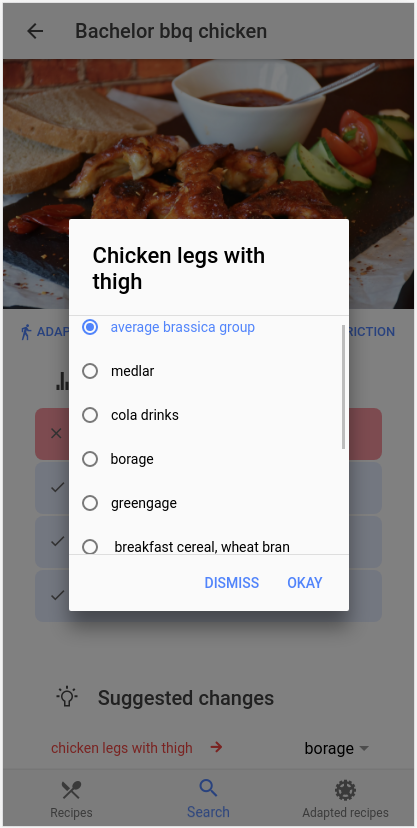
\includegraphics[width=\linewidth]{imagenes/app/pantallas/ejemplo15.png}
        \caption{Adaptando receta II}
        \label{fig:ejemplo15}
    \end{subfigure}
    \caption{Adaptación de una receta vegetariana}
    \label{fig:seleccion2}
\end{figure}

% Con los ejemplos mostrados en este apartado hemos podido comprobar las ventajas de utilizar el modelo predictivo implementado para poder adaptar dietas, puesto que la semántica capturada en el modelo permite alcanzar buenas alternativas a los elementos restringidos. Por otra parte, se ha podido ver la interpretabilidad de este módulo, ya que paso a paso se indican aquellos ingredientes no adecuados y que deben ser sustituidos por otros. 